\section{Evaluation}
\label{sec:experiments}

\subsection{Setup}
\label{sec:setup}

\paragraph{Models, Hardware, Frameworks.}
We evaluate \textbf{Qwen3-32B} and \textbf{Qwen3-4B} (dense)~\citep{yang_qwen3_2025} and
\textbf{Qwen3.5-35B-A3B} (a 3B-active mixture-of-experts)~\citep{qwen_qwen35_2026} to
test generalization across both scale and architecture, all self-hosted via
vLLM~0.19.1 (TP=1) on NVIDIA H20-3e GPUs (143\,GiB each) with bf16 precision.
All runs use greedy decoding (temperature~0, seed~42) with thinking mode enabled,
producing 2--20\,s of chain-of-thought decode that creates the overlap budget \spork{} exploits.

\paragraph{Benchmarks.}
Table~\ref{tab:benchmarks} (Appendix~\ref{app:configs}) profiles the three benchmarks.
GAIA and HotpotQA execute \emph{real} network tools (web search + page browse, and a
Wikipedia search API, respectively); tau2-bench executes structured DB-query tools with
simulated latency floors, giving a controlled sweep over $\Ttool$.

\paragraph{Metrics.}
\textbf{Latency}: per-query end-to-end wall-clock time.
\textbf{Quality}: exact-match accuracy (EM) for GAIA/HotpotQA, F1 for HotpotQA.
\textbf{Speedup}: $P_{95}$ ratio (baseline / \spork{}).

\paragraph{Configurations.}
Per-model serving mode, baseline, and \spork{} configuration appear in
Table~\ref{tab:configs} (Appendix~\ref{app:configs}); the dense-model baseline is
vLLM's built-in ngram speculative decoding~\citep{saxena_pld_2023}, and each model is
compared against its own baseline under the same serving mode.

\subsection{End-to-End Speedup}
\label{sec:e2e_speedup}

Figure~\ref{fig:hero_speedup} reports end-to-end $P_{95}$ latency across models and
benchmarks.
With Qwen3-32B, \spork{} achieves \textbf{$-$18\% $P_{95}$} on GAIA (131.9\,s $\to$
108.1\,s, real web search, $\Ttool = 4.8$\,s), while HotpotQA shows a modest
1.06$\times$ improvement because its short tools ($\Ttool = 0.9$\,s) sit near the EQ1
break-even.
The benefit transfers across model \emph{size}: Qwen3-4B achieves \textbf{1.15$\times$}
mean speedup on tau2-bench (simulated 2\,s tool floor), with full benchmark coverage in
Appendix~\ref{app:qwen4b}.
It also transfers across model \emph{architecture}: Qwen3.5-35B-A3B reduces $P_{95}$ by
16\% on tau2 (59.4\,s $\to$ 49.8\,s, N=155), 16\% on GAIA (222.4\,s $\to$ 187.3\,s,
N=53, tail-positive), and 20\% on HotpotQA (18.9\,s $\to$ 15.2\,s, N=200).

\begin{figure}[t]
  \centering
  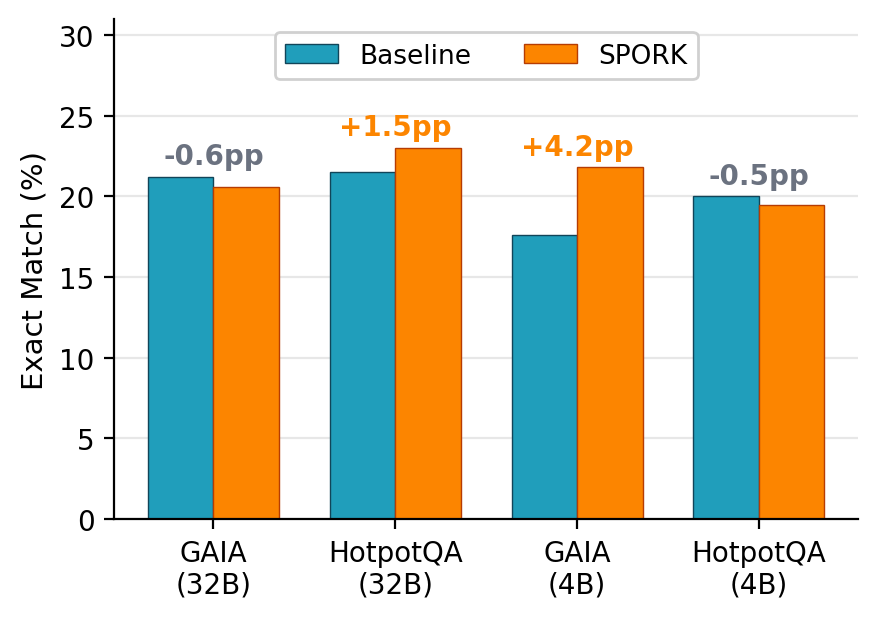
\includegraphics[width=0.92\columnwidth]{figures/fig_quality_preservation.png}
  \caption{\textbf{\spork{} preserves task accuracy.} Paired comparison of baseline (teal)
  vs.\ \spork{} (orange) exact-match scores across benchmarks and model sizes.
  Quality stays within 1\,pp of baseline on all settings and sometimes improves
  (+1.5\,pp EM on HotpotQA with Qwen3-32B). The strict gate prevents speculative side
  effects from corrupting conversation history.}
  \label{fig:quality}
\end{figure}


\spork{} achieves $-$18\% $P_{95}$ on GAIA (Qwen3-32B) and 1.15$\times$
mean on tau2 (Qwen3-4B), confirming that the overlap window dominates when
tool latency $\geq$ 2\,s. \S\ref{sec:envelope} locates these points in the EQ1 envelope.

\subsection{Quality Preservation}
\label{sec:quality}

We expect \spork{} to preserve task accuracy: the strict gate ensures only
exact-matching tool calls are accepted, and D3 recycles only the rejected probe's
verified prefix as a speculative-decoding draft.
Speculative decoding's verification step preserves the target model's output
distribution~\citep{leviathan_fast_2023}; in \spork{} the target is the running model
itself, so D3 inherits this guarantee.

Figure~\ref{fig:quality} shows that \spork{} keeps EM within 1\,pp of baseline on
every benchmark and model, and sometimes improves it.
tau2-bench is not plotted because its quality is identical by construction: the
simulated DB tools return deterministic canned results, matching exactly for baseline
and \spork{}, so the latency sweep exercises timing only.
GAIA and HotpotQA instead call search APIs whose results are non-deterministic even
under identical arguments, so baseline and \spork{} trajectories cannot be
token-identical despite temperature~0; quality on these benchmarks is therefore
compared via aggregate scores (EM, F1) rather than per-token equality.
On HotpotQA with Qwen3-32B, \spork{} is faster
\emph{and} higher quality (+1.5\,pp EM, +0.012 F1) than the baseline.

\spork{} preserves accuracy (within $-$1\,pp of baseline) regardless of model size or
benchmark.
The strict gate is the key mechanism: it rejects any probe that does not exactly match
the main generation, ensuring the conversation history is never corrupted by speculative
side effects.

\subsection{Ablation}
\label{sec:ablation}

We expect each component (D1, D2, D3) to contribute independently to the final result,
with no single configuration dominating all metrics simultaneously.

\begin{figure}[t]
  \centering
  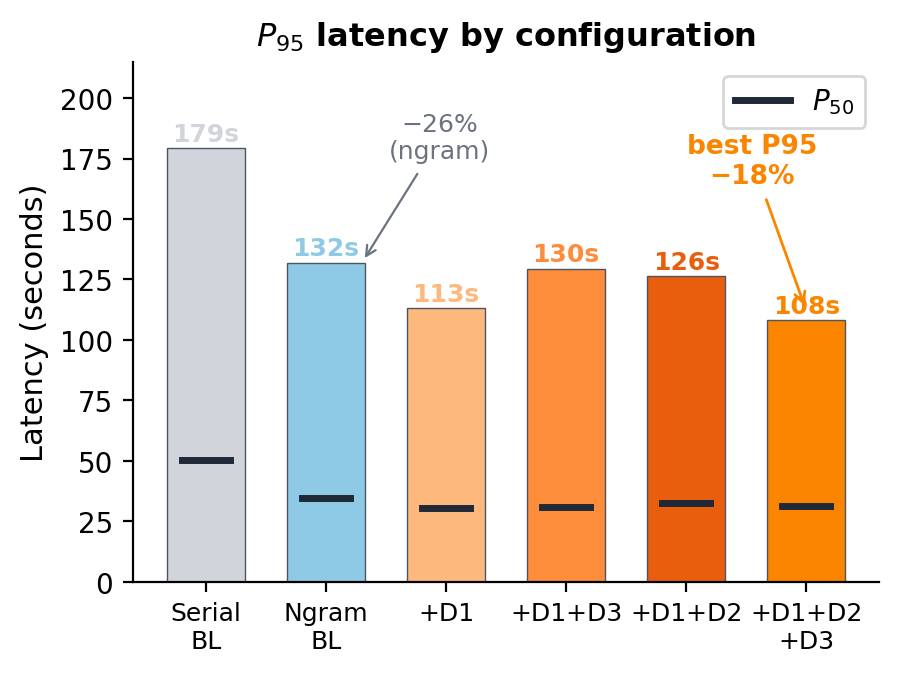
\includegraphics[width=0.92\columnwidth]{figures/fig_ablation_decomposition.png}
  \caption{\textbf{Ablation: full \spork{} (D1+D2+D3) achieves the best tail latency.}
  GAIA N=165, Qwen3-32B; black dashes mark $P_{50}$.
  Ngram alone gives $-$31\% at $P_{50}$; D1+D2+D3 adds $-$18\% at $P_{95}$.
  No single config wins on all metrics: D1 for mean, D1+D2+D3 for $P_{95}$.}
  \label{fig:ablation}
\end{figure}

Figure~\ref{fig:ablation} decomposes contributions:
\begin{itemize}
  \item \textbf{Ngram spec-dec (the baseline)}: accelerates decode TPOT
    ($P_{50}$ 50.5$\to$34.7\,s, $-$31\%); every \spork{} configuration stacks on top of
    it, so the contributions below are orthogonal to token-level speculative decoding.
  \item \textbf{D1 on ngram}: additional $P_{50}$ $-$12\%, mean $-$10\%. Fork-prefix
    overlap adds on top of per-token spec-dec.
  \item \textbf{D1+D2+D3}: best $P_{95}$ (108.1\,s, $-$18\%). D2+D3 synergy helps
    tail queries where rejected retries leave verified prefixes that D3 recycles as
    drafts.
\end{itemize}

Per-configuration EM differences exist but stem from search-API and vLLM-batching
nondeterminism, both present in the baseline as well (\S\ref{sec:quality}); they do not
originate from the gate: D3 accepts only tokens that match the main model's greedy
output, so trajectory divergence is orthogonal to \spork{}'s correctness guarantee.

\parabf{D2 confidence gate analysis.}
D2 is a trade-off knob.
The gate raises per-turn acceptance from $\alpha \approx 0.22$ (D1, 49 accepted probes)
to $\alpha \approx 0.37$ (D1+D2, 101 accepted) and avoids wasted real tool calls by
filtering low-confidence probes before dispatch; the dispatched-probe totals (434 for
D1, 2124 for D1+D2) exceed the turn counts because the retry cadence re-probes
low-confidence turns (\S\ref{sec:eq1}).
The confidence threshold $\theta=0.90$ was selected by sweeping min-prob over 997 probes:
precision 88\%, recall 100\%, F1$=$0.937 (Figure~\ref{fig:d2_gate}).
This filtering pays when tools are slow or costly; when tools are cheap, the added wait
can outweigh the savings, and D2 alone can hurt mean latency on short-tool benchmarks.
With D3, the gate's rejected retries become useful drafts, and D2+D3 together give the
best $P_{95}$: the full configuration wins the tail while D1 alone wins the mean.

Each component contributes to different metrics: D1 for mean/P50, D2+D3 for $P_{95}$.
All three are needed for the best tail latency.

\subsection{Case Study: Self-Speculation vs.\ a Draft Model}
\label{sec:case_study}

\begin{figure}[t]
  \centering
  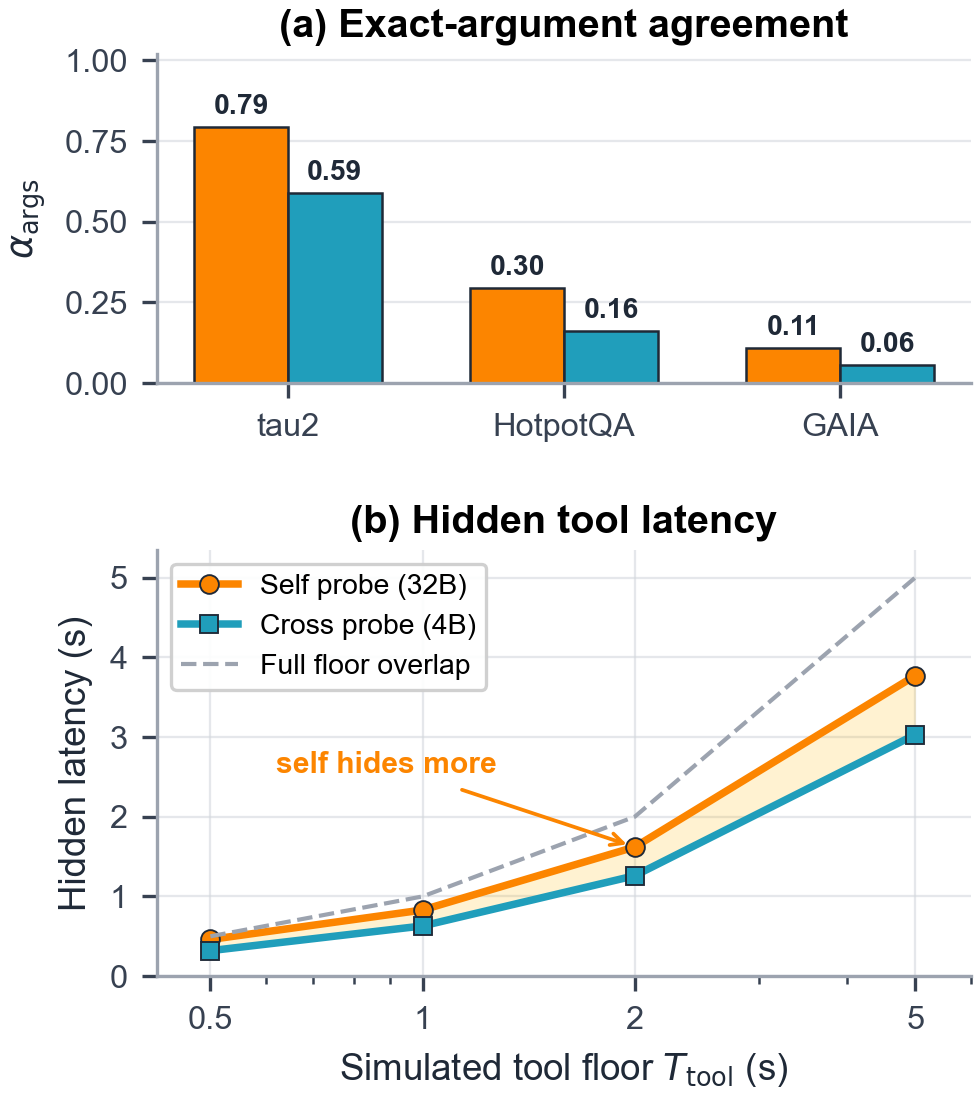
\includegraphics[width=0.92\columnwidth]{figures/fig_self_vs_cross4b_ablation.png}
  \caption{\textbf{Self-speculation trades a slower probe for higher useful overlap.}
  D1-only HTTP ablations with the same Qwen3-32B main model.
  \textit{(a)}~Self has higher exact-argument agreement than a Qwen3-4B cross probe
  on all three benchmarks.
  \textit{(b)}~On tau2, self hides more mean tool latency across floors; cross wastes
  2.1$\times$ more speculative tools at the 2\,s floor.}
  \label{fig:self_cross_ablation}
\end{figure}

A natural alternative to self-speculation is to serve a smaller model as a tool-call
drafter, analogous to token-level speculative decoding.
Figure~\ref{fig:self_cross_ablation} compares that
choice against self-speculation in a controlled D1-only HTTP ablation on tau2-bench:
same Qwen3-32B main model, tasks, seed, parser, and simulated tool floor; only the probe
model changes.

The cross-4B probe has lower probe latency, the time to decode the tool-call token
span: 0.315\,s mean vs.\ 0.970\,s for self at the tau2 2\,s floor.
Its exact-argument agreement, however, is far lower than self-speculation's: 0.590
vs.\ 0.792 on tau2 (Figure~\ref{fig:self_cross_ablation}\textit{a}), 0.161 vs.\ 0.296
on HotpotQA, and 0.056 vs.\ 0.109 on GAIA.
Since both probes usually finish before the tool floor on accepted turns, probe speed is
off the critical path; acceptance rate dominates realized overlap.
Self-speculation therefore hides more tool latency at every floor in the sweep and wastes
fewer speculative tool executions (154 vs.\ 317 at N=155;
Figure~\ref{fig:self_cross_ablation}\textit{b}).
It also avoids a second served model: in our measurement the cross-model arm serves two
models (Qwen3-32B and the Qwen3-4B drafter, each TP=1 on its own GPU), while
self-speculation needs only the target model's single GPU; a colocated drafter would
instead compete with the target for request scheduling and KV-cache capacity.
This result places a boundary on external drafters: they help only if their lower probe
cost offsets the lower $\alpha$ and the additional serving contention.

\subsection{Operating Envelope}
\label{sec:envelope}

We expect \spork{} to break even when tool latency exceeds probe overhead
($\Ttool \geq \Toh$, the probe overhead of \S\ref{sec:d1}) and the model produces
sufficient CoT for overlap.
Below this threshold, probe overhead dominates and \spork{} is neutral or negative.

\parabf{EQ1 calibration.}
The tau2 latency sweep validates EQ1's structural prediction: speedup grows monotonically
with tool latency (1.09$\times$ at 0.5\,s floor $\to$ 1.18$\times$ at 5.0\,s floor on
airline domain).
EQ1 predicts observed speedup with at most 1.84\% residual across all operating points
(1.84\% on tau2, 0.88\% on GAIA), confirming the cost model is a reliable predictor of
when \spork{} helps.

\begin{figure}[t]
  \centering
  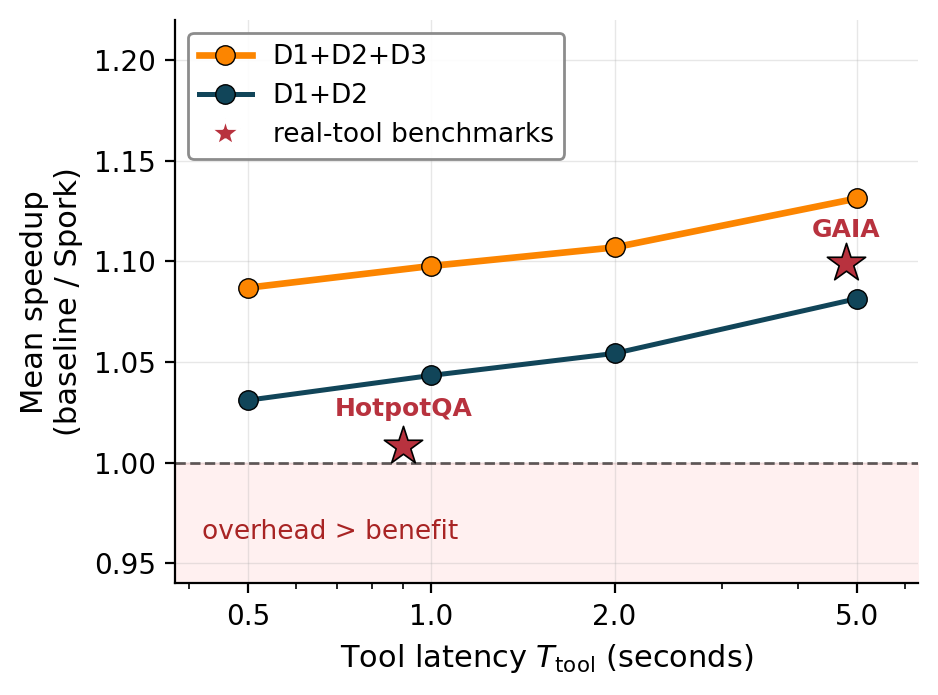
\includegraphics[width=0.92\columnwidth]{figures/fig_operating_regime_map.png}
  \caption{\textbf{\spork{} stays at or above break-even across the operating envelope.}
  Mean per-task speedup vs.\ tool latency on the tau2 sweep (N=155). Full \spork{}
  (D1+D2+D3) stays above break-even and rises with tool latency; the gated D1+D2 line
  approaches break-even on the shortest floors, matching EQ1's
  $\alpha\cdot\toverlap \geq \Toh$ condition.
  Stars mark the two real-tool operating points (Qwen3-32B mean speedup): near-neutral
  HotpotQA at EQ1's break-even, GAIA well inside the beneficial region.}
  \label{fig:operating_regime}
\end{figure}

Figure~\ref{fig:operating_regime} traces this envelope on the controlled tau2 sweep.
The real-tool benchmarks land where the cost model places them: GAIA's 4.8\,s tool
latency sits well inside the beneficial region, while HotpotQA's 0.9\,s latency sits
near break-even, exactly where EQ1 predicts the gains should shrink toward neutrality.

\parabf{When \spork{} wins.}
The largest gains appear when $\Ttool$ is large relative to probe overhead, tool schemas
are regular enough for high $\alpha$, and speculation is restricted to read-only
tools (\S\ref{sec:implementation}): GAIA's multi-second real web search is the
clearest favorable regime ($P_{95}$ $-$18\%).
On HotpotQA (0.9\,s Wikipedia API), \spork{} is Pareto-dominant with Qwen3-32B (faster and
higher EM) and Pareto-neutral with Qwen3-4B: it never hurts, and occasionally helps on
tail queries.
The case study (\S\ref{sec:case_study}) reinforces the principle: once the probe finishes
before the tool floor, acceptance rate, not probe speed, determines hidden tool latency.

\parabf{When \spork{} does not help.}
The primary boundary is a vanishing overlap window ($\toverlap \to 0$): from the decode
side, no-think mode cuts main decode to 0.3--0.9\,s, too fast for the probe to finish
before the main stream needs the tool result (0.79$\times$ on tau2), while thinking-mode
CoT, typically $\geq$2\,s in our workloads, creates the window; from the tool side, very
fast tools (e.g., local file reads) finish before any probe can pay off, leaving nothing
to hide.
The window also bounds long tools: $\toverlap$ ends when either side finishes, so tool
time that runs past the main stream's stop is not hidden, and the relative gain
saturates once $\Ttool$ exceeds the decode remaining at dispatch.
A second boundary, a native tool-call format that diverges from the forced probe
($\alpha \to 0$), is detailed in Appendix~\ref{app:format_divergence}.

\spork{}'s operating boundary is well-defined: thinking-mode CoT long enough to host the
probe, and tool latency above the probe-overhead break-even, with gains growing until
$\Ttool$ fills the available decode window.
Practitioners can evaluate applicability before full deployment with a lightweight pilot
trace measuring fork name accuracy, $\alpha$, and $\Ttool$, plugged into EQ1.

\FloatBarrier
